\chapter[Modelos e resultados]{Modelos e resultados}\label{sec:modelos}

Neste capítulo, serão apresentados os modelos neurais utilizados e a parametrização realizada tanto para eles quanto para o SVM.

\section{Modelo de ML}

O modelo SVM foi o escolhido para servir de linha de base para comparação com os demais modelos. Visto que o BoW e SVM juntos possuem bons resultados para classificação de textos mais longos \cite{wang_baselines_2012}.

Para parametrizar o modelo, foi utilizada a base de validação, portanto, escolheu-se o modelo com os parâmetros que apresentasse melhores resultados neste conjunto de dados. Vale notar que, ao mesmo tempo em que busca-se ótimos resultados na validação, os modelos com casos de \textit{overfitting}, ou seja, o modelo prediz com uma alta taxa a base de treino, foram desconsiderados. Além disso, os parâmetros foram variados de acordo com o disponível na implementação do \citeonline{pedregosa_scikit-learn:_2011}.

Para encontrar os melhores parâmetros do modelo, seguiu-se as recomendações de \citeonline{wang_baselines_2012}. Utilizou-se os núcleos Linear, RBF e Polinomial de segunda ordem. Combinados a ele fez-se um balanceamento de classes e seleção da contante C em 1.0 padrão \cite{pedregosa_scikit-learn:_2011} e 0.1 para maior controle do \textit{overfitting} \cite{wang_baselines_2012}. Foi utilizado 4 variações diferentes do dado para o SVM: Formato de símbolos pré-processado e não pré-processado, BoW também pré-processado e não pré-processado. Os melhores resultados para seleção de parâmetros estão na Tabela \ref{tab:svmParametros}, para os demais não listados, utilizou-se os valores padrão da implementação.

\begin{table}[ht]
    \centering
    \caption[Resultados e parâmetros do SVM]{Resultados no conjunto de validação e sua respectiva parametrização e processamento de dados.}
    \label{tab:svmParametros}
    \begin{tabular}{|c|c|c|c|c|c|c|}
        \hline 
        Acurácia & Transformação & Pré-processado & Núcleo & C & Grau & Balanceamento\protect\footnotemark \\
        \hline 
        0,5003 & símbolos & X & polinomial & 1,0 & 2 & - \\
        \hline 
        0,4167 & símbolos & - & RBF & 0,1 & - & X \\
        \hline 
        \textbf{0,9178} & \textbf{BoW} & \textbf{X} & \textbf{linear} & \textbf{0,1} & \textbf{1} & \textbf{X} \\
        \hline 
        0,9126 & BoW & - & linear & 0,1 & 1 & X \\
        \hline
    \end{tabular}\par Fonte: elaboração própria.
\end{table}

\footnotetext{O balanceamento foi computado utilizando o método da biblioteca do Scikit Learn de \citeonline{pedregosa_scikit-learn:_2011} \textit{sklearn.utils.class\_weight.compute\_class\_weight}}

\section{Modelos neurais}

Modelos hierárquicos como Hierarchical Attention Network  \cite{yang_hierarchical_2016} e CNN/LSTM-GRNN \cite{tang_document_2015} foram inviabilizados, pela dificuldade de determinar quando uma sentença se inicia no documento, visto que o processo de extração de dados não deixou o conteúdo livre de caracteres especiais ou lixos. Assim, utilizar separadores de sentença pré-treinados não foi possível pela quantidade sentenças irregulares resultantes. Os terminadores de períodos comuns geraram confusão em muitos documentos.

%Dos modelos neurais, utilizou-se os modelos MLP, LSTM \cite{hochreiter_long_1997}, BLSTM \cite{braz_document_2018}, BRNN \cite{schuster_bidirectional_1997}, CNN \cite{da_silva_document_2018}, CNN-rand \cite{kim_convolutional_2014}, VDCNN \cite{conneau_very_2017}, BLSTM-C \cite{lai_recurrent_2015} e C-LSTM \cite{zhou_c-lstm_2015} como base. Eles foram modificados a medida do necessário para ajustar a quantidade de dados e melhorar suas performances baseadas nas métricas de Acurácia, Precisão e Revocação.

Para todas as redes utilizadas, o vetor de enviesamento foi inicializado com o valor 0, a função de otimização utilizada foi a \textit{Adam} com a taxa de aprendizado
de 0.001 e valores \textit{beta1} e \textit{beta2} com 0.9 e 0.9999 respectivamente. 

Não foram utilizadas funções de regularização, decaimento da taxa de
aprendizado, nem diferenciação dessa taxa entre diferentes camadas.

A MLP foi utilizada em todas as arquiteturas como camada de saída com 6 neurônios, uma
unidade para cada categoria de documento. Utilizou-se também a função de ativação \textit{softmax},
e a função para cálculo de \textit{loss}  foi o \textit{categorical
cross entropy}.

Escolheu-se o tamanho 256 para os mini lotes (do inglês \textit{mini batch}) de treinamento com 30 épocas (do inglês \textit{epochs}). Salvou-se vários estados intermediários da rede neural durante o treinamento com os pesos que geraram a melhor acurácia. Dessa forma, na hora de coletar o resultado na base de treino, fez-se o carregamento destes melhores pesos.

\subsection{\textit{Multilayer Perceptron}}

\begin{figure}[ht]
    \centering
    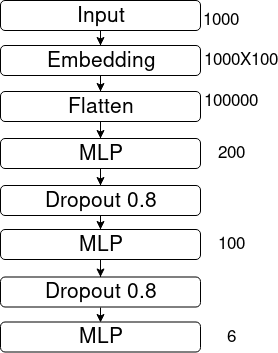
\includegraphics[keepaspectratio=true,scale=0.5]{figuras/modelos-Dense}
    \caption[Modelo MLP]{Representação gráfica do modelo neural denso com três camadas ocultas, uma de entrada e uma de saída. Fonte: elaboração própria.}
    \label{fig:mlp}
\end{figure}

Elaborou-se um modelo de \textit{Multilayer Perceptron} (\textbf{MLP}), como apresentado na Figura \ref{fig:mlp} para servir de base de comparação dos demais algorítmos. No diagrama está presente duas camadas ocultas de MLP com 200 e 100 células cada, seguidas de \textit{dropout} de 0.8. A função de ativação utilizada foi a ReLu..


\subsection{Recorrente}

\begin{figure}[ht]
    \centering
    \begin{subfigure}[b]{0.35\textwidth}
        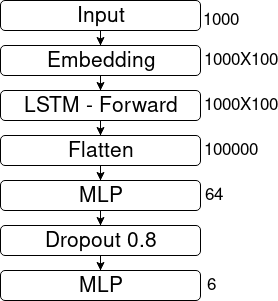
\includegraphics[width=\textwidth]{figuras/modelos-LSTM}
        \caption{Modelo baseado em LSTM \newline \cite{hochreiter_long_1997}.}
        \label{fig:lstm}
    \end{subfigure}\hfill
    \begin{subfigure}[b]{0.4\textwidth}
        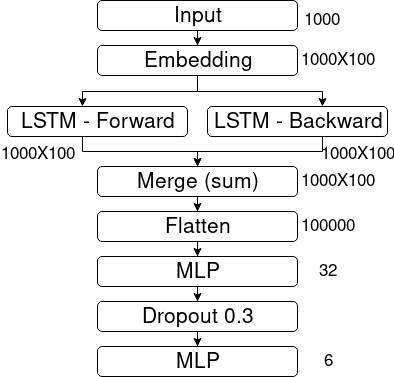
\includegraphics[width=\textwidth]{figuras/modelos-BLSTM}
        \caption{Modelo baseado em \textit{Bidirectional} LSTM \cite{braz_document_2018}.}
        \label{fig:blstm}
    \end{subfigure}
    \begin{subfigure}[b]{0.45\textwidth}
        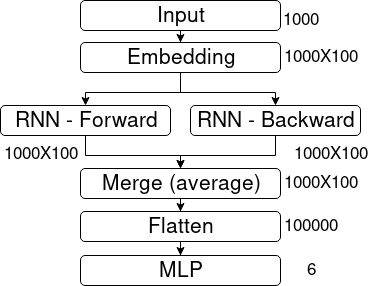
\includegraphics[width=\textwidth]{figuras/modelos-BRNN}
        \caption{Modelo baseado em \textit{Bidirectional} RNN \cite{schuster_bidirectional_1997}.}
        \label{fig:brnn}
    \end{subfigure}
    \caption[Modelos recorrentes]{Representações gráficas para os modelos neurais recorrentes.}
\end{figure}


Os modelos recorrentes foram utilizados na sua forma padrão, em que a saída de cada neurônio retorne um valor para a próxima camada, ao invés de apenas um número ao final da sequência da camada \cite{goldberg_neural_2017}, ou que a saída de uma célula se torne a entrada da próxima \cite{goldberg_neural_2017} na mesma camada, nem fez-se uso das técnicas de atenção \cite{goldberg_neural_2017} as quais fazem o modelo manter um vetor adicional para priorizar um conjunto de palavras na saída da rede.
 
Para o modelo \textit{Long Short-Term Memory} (\textbf{LSTM-pre}) \cite{hochreiter_long_1997} foi necessário o texto pré-processado, pois sem ele, o modelo não foi capaz de generalizar todas as classes, predizendo sempre uma ou duas. Utilizou-se 100 células com uma taxa de \textit{dropout} de 0.5. Foi adicionado mais uma rede MLP com 64 neurônios. A representação das camadas deste modelo estão na Figura \ref{fig:lstm}.

Os modelos Bidirecionais Recorrentes possuem a sua estrutura semelhante, a diferenciação é o algorítmo da célula de cada um deles \cite{graves_framewise_2005}. Utiliza-se da propriedade do modelo recorrente, e treina-se duas camadas, uma com os dados na sequência direta e outra reversa. Dessa forma, consegue-se obter contexto de $x_{i-1}$ e $x_{i+1}$ na unidade da posição $x_i$.

Para a arquitetura do modelo da \textit{Bidirectional Recurrent Neural Network} (\textbf{BRNN-pre}) \cite{schuster_bidirectional_1997},
utilizou-se 100 unidades recorrentes, retornando os valores de saída de cada
neurônio com um fator de \textit{dropout} de 0.2 a fim de minimizar o \textit{overfitting} no
treino com muitos \textit{epochs}. Ao modelo foi adicionada uma camada de \textit{Embedding} com
vetor de saida de tamanho 100. A função de mescla, foi a média aritmética dos
vetores de saída. O modelo está representado na Figura \ref{fig:brnn}. Para o
resultado desta arquitetura, foi necessário utilizar o texto pré-processado, pois
sem ele, a rede não conseguia generalizar todas as classes.

Ao modelo \textit{Bidirectional Long Short-Term Memory} (\textbf{BLSTM}) \cite{braz_document_2018}, foi adicionado uma camada de MLP com \textit{dropout} de valor 
0.3. Foram utilizados 100 células de memorização em cada LSTM. A mescla dos resultados foi feito com a média dos vetores de saída. A representação das camadas
deste modelo estão na Figura \ref{fig:blstm}.

\subsection{Convolucional}

\begin{figure}
    \centering
    \begin{subfigure}[b]{0.25\textwidth}
        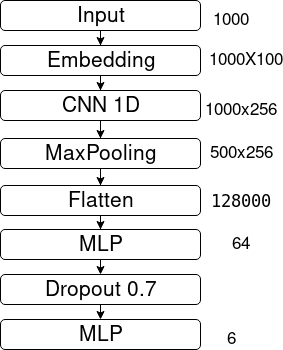
\includegraphics[width=\textwidth]{figuras/modelos-CNN}
        \caption{Modelo baseado em CNN \cite{da_silva_document_2018}.}
        \label{fig:cnn}
    \end{subfigure}\hfill
    \begin{subfigure}[b]{0.4\textwidth}
        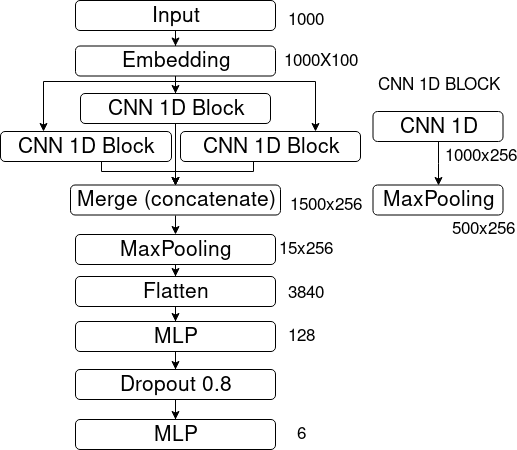
\includegraphics[width=\textwidth]{figuras/modelos-CNN-rand}
        \caption{Modelo baseado em CNN \cite{kim_convolutional_2014}.}
        \label{fig:cnnrand}
    \end{subfigure}\hfill
    \begin{subfigure}[b]{0.5\textwidth}
        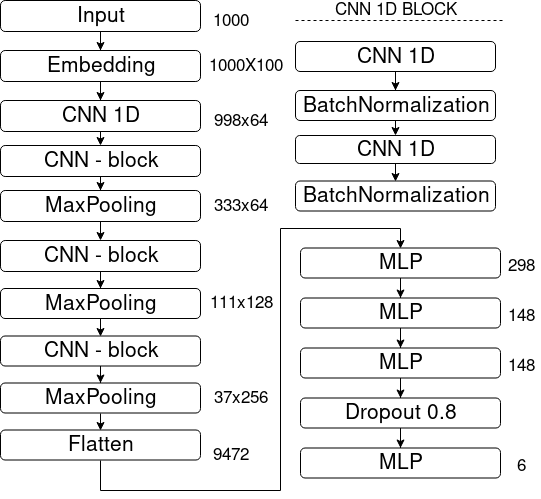
\includegraphics[width=\textwidth]{figuras/modelos-VDCNN}
        \caption{Modelo baseado em CNN \cite{conneau_very_2017}.}
        \label{fig:vdcnn}
    \end{subfigure}
    \caption[Modelos convolucionais]{Representações gráficas para os modelos neurais convolucionais.}
\end{figure}

O modelo \textit{Convolutional Neural Network} (\textbf{CNN}) \cite{da_silva_document_2018} é uma implementação simples do modelo com apenas uma convolução
seguida de um \textit{max pooling}, seguida da rede MLP com 64 neurônios e com
dropout de 0.7. O propósito deste modelo é servir como linha de base para os
modelos convolucionais mais complexos utilizados. Diferentemente do modelo proposto apresentado por \citeauthor{da_silva_document_2018} \citeyear{da_silva_document_2018}, foi utilizado apenas a primeira página, isso fez com que a contagem de símbolos é inferior a 1000, assim o tamanho do vetor de entrada foi reduzido. Também foi adicionada uma camada escondida de MLP com \textit{dropout} como apresentado na \ref{fig:cnn}, os demais parâmetros foram mantidos.

O modelo \textit{Convolutional Neural Network} (\textbf{CNN-rand}) \cite{kim_convolutional_2014} foi modificado adicionando-se um
dropout de 0.4 em cada canal de convolução. Realizar o treinamento do zero dos \textit{embeddings} de uma CNN não geram os melhores resultados \cite{kim_convolutional_2014}, entretanto não encontrou-se um modelo de \textit{embedding} na língua portuguesa publicado em artigo que pudesse ser retreinado. A convolução foi feita com núcleos de
tamanhos 3,4 e 5 e um total de 256 filtros, concatenando zeros para manter o tamanho do
vetor ao final da convolução. O \textit{max pooling} foi obtendo o maior valor
de uma janela de tamanho 2. Após a concatenação o \textit{max pooling} aplicado
foi com uma janela de tamanho 100. A representação deste modelo está na Figura
\ref{fig:cnnrand}.

O \textit{Very Deep Convolutional Neural Network} (\textbf{VDCNN}) \cite{conneau_very_2017} foi reparametrizado para trabalhar com a carga de dados deste trabalho,
portanto, foi removido um bloco de convolução, utilizando-se apenas 64, 128 e
256 filtros. Cada bloco desse foi montado com duas convoluções de núcleo com
tamanho 3 e adicionada uma normalização, para garantir que os desvios padrões das taxas de ativação
sejam próximas de 1. O \textit{max pooling} dos blocos de convolução, são com
janela de tamanho 2 e avanço de 3. O modelo está representado na Figura
\ref{fig:vdcnn}.



\subsection{Modelos mistos}

\begin{figure}[ht]
    \centering
    \begin{subfigure}[b]{0.4\textwidth}
        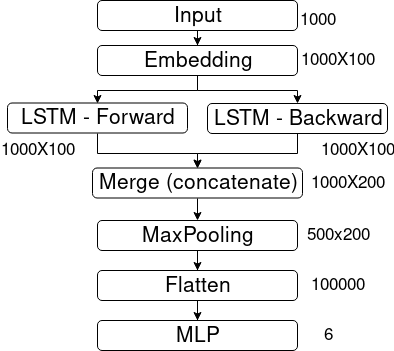
\includegraphics[width=\textwidth]{figuras/modelos-BLSTM-C}
        \caption{Modelo baseado em BLSTM-C \cite{lai_recurrent_2015}.}
        \label{fig:blstmc}
    \end{subfigure}\hfill
    \begin{subfigure}[b]{0.3\textwidth}
        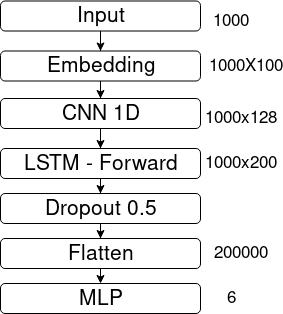
\includegraphics[width=\textwidth]{figuras/modelos-C-LSTM}
        \caption{Modelo baseado em CNN-LSTM \cite{zhou_c-lstm_2015}.}
        \label{fig:clstm}
    \end{subfigure}
    \caption[Modelos mistos]{Representações gráficas para os modelos neurais combinados entre convolucionais e recorrentes.}
\end{figure}

O modelo \textit{Bidirectional Long Short-Term Memory-Convolutional} (\textbf{BLSTM-C}) \cite{lai_recurrent_2015} é uma BLSTM que possui um
\textit{max pooling} para extrair as melhores features da saída das LSTM,
portanto na mesca dos resultados, é utilizado a concatenação. O modelo está
representado na Figura \ref{fig:blstmc}.

O \textit{Convolutional Neural Network Long Short-Term Memory} (\textbf{C-LSTM}) \cite{zhou_c-lstm_2015} é uma proposta de utilizar a CNN como extratora
de características e utilizar este mapa de características na LSTM, assim como
representado na Figura \ref{fig:clstm}. A convolução possui 128 filtros com
núcleo de tamanho 2, a LSTM tem 200 células.


\section{Resultados dos modelos}

A seguir nesta seção, serão apresentados os resultados do treinamento e predição do conjunto de teste. Nas tabelas e gráficos estão presentes as métricas coletadas para avaliar a performance do modelo e outras auxiliares.

\subsection{Treinamento e validação}

A execução dos modelos acima propostos foi no \textit{hardware} NVidia\footnote{Esta placa de vídeo foi doação da compania NVidia ao projeto GPAM para realização em pesquisas de ML.} TitanXP 12 GB 3840 Cuda Cores a 1.5 GHz, Intel Core i5 7400, 48 GB DDR4 2133MHz, obteve-se os resultados da Tabela \ref{tab:execucaoModelos}. Para gerar os tempos no conjunto de treinamento e de teste foram consideradas as quantidades de amostras apresentadas na Tabela \ref{tab:categoriasPecas}.

\begin{table}[ht]
    \centering
    \caption[Resultados dos modelos classificadores nos conjuntos de treino e validação]{Dados da execução dos modelos classificadores nos conjuntos de treino e validação.}
    \label{tab:execucaoModelos}
    \begin{tabular}{|c|c|l|l|c|}
        \hline
        Modelo & Melhor Epoch & Treinamento & Teste & pré-processamento \\
        \hline
        \textbf{MLP} & \textbf{28} & \textbf{0m 1s 2ms 822us} & \textbf{0s 121us} & \textbf{0} \\
        \hline
        LSTM-pre & 9 & 38s 10ms 071us & 1s 1ms & 4s 58ms  \\
        \hline
        BLSTM & 3 & 91s 17ms 925us & 1s 1ms & 0 \\
        \hline
        BRNN-pre & 20 & 34s 61ms 0us & 7s 10ms & 4s 58ms \\
        \hline
        CNN & 21 & 34s 6ms 756us & 2s 4ms & 0 \\
        \hline
        VDCNN & 24 & 44s 18ms 455us & 1s 2ms & 0 \\
        \hline
        CNN-rand &	20 & 91s 21ms 546us & 5s 7ms & 0 \\
        \hline
        BLSTM-C	& 9 & 96s 20ms 229us & 2s 3ms & 0 \\
        \hline
        C-LSTM & 6 & 91s 21ms 447us & 6s 8ms & 0 \\
        \hline
        SVM Linear-pre & - & 6s 72ms 0us & 1s 31ms & 4s 58ms \\
        \hline
        SVM Linear & - &  11s 100ms 0us & 2s 100ms & 0\\
        \hline
    \end{tabular}\par Fonte: elaboração própria.
\end{table}

A utilização das bibliotecas de aprendizado profundo Keras\footnote{Biblioteca que facilita a criação de diferentes arquiteturas neurais, faz uso de \textit{backends} de processamento tanto em GPU quanto CPU. Disponível em: <https://keras.io/>. Acessado em: 25 de Novembro de 2018} e de processamento Tensforflow\footnote{Um \textit{framework} \textit{open source} de aprendizado de máquina que viabiliza computação numérica de alta performace. Disponível em: <https://www.tensorflow.org/>. Acessado em: 25 de Novembro de 2018.} que possuem implementações otimizadas para placa de vídeo, possibilitaram que todos os tempos de execução na Tabela \ref{tab:execucaoModelos} fossem abaixo de 1 minuto e 40 segundos. Ressalta-se que para os modelos SVM Linear, LSTM e BRNN, os quais utilizaram dados pré-processados, deve-se considerar o tempo adicional de tratamento do dado. Dessa forma os tempos para esses modelos são $10s\ 13ms$, $42s\ 68ms\ 071us$ e $38s\ 119ms$ respectivamente, para seus tempos de teste adiciona-se $580ms$ ficando $1s\ 621ms$, $1s\ 581ms$ e $7s\ 590ms$.

\begin{figure}[ht]
    \centering
    \begin{subfigure}[b]{0.5\textwidth}
    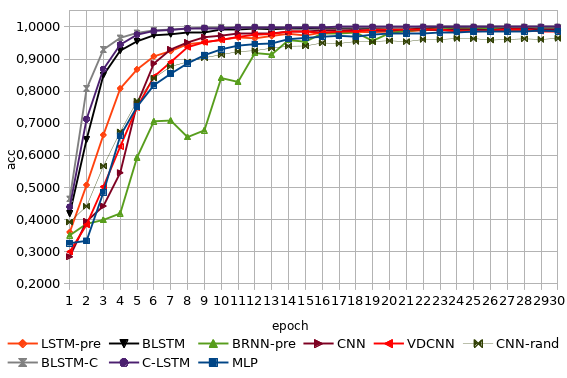
\includegraphics[width=\textwidth]{figuras/treinoacc}
        \caption{Conjunto de treino}
        \label{fig:acc}
    \end{subfigure}\hfill
    \begin{subfigure}[b]{0.5\textwidth}
        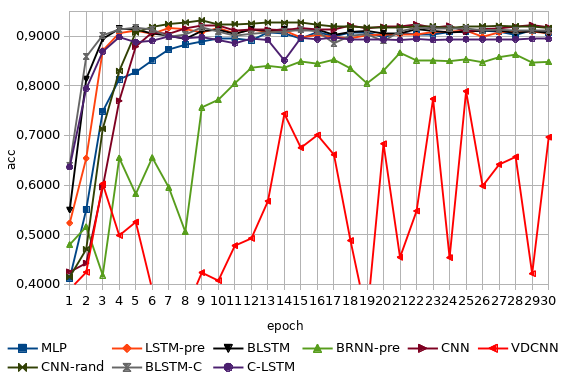
\includegraphics[width=\textwidth]{figuras/valacc}
        \caption{Conjunto de validação}
        \label{fig:valacc}
    \end{subfigure}
    \caption[Acurácia dos modelos neurais]{Acurácia dos modelos neurais durante a fase de treinamento e validação, separados por cada \textit{epoch}. Fonte: elaboração própria.}
    \label{fig:tvacc}
\end{figure}

\begin{figure}[ht]
    \centering
    \begin{subfigure}[b]{0.5\textwidth}
        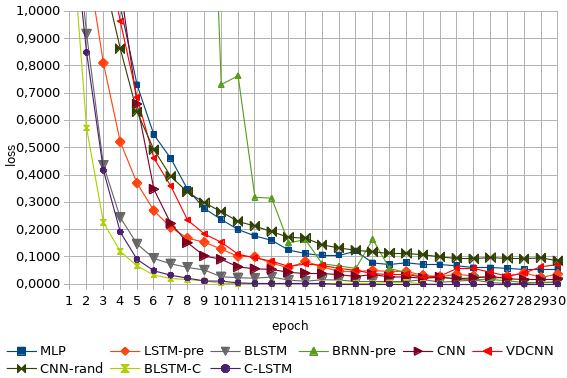
\includegraphics[width=\textwidth]{figuras/treinoloss}
        \caption{Conjunto de treino}
        \label{fig:loss}
    \end{subfigure}\hfill
    \begin{subfigure}[b]{0.5\textwidth}
        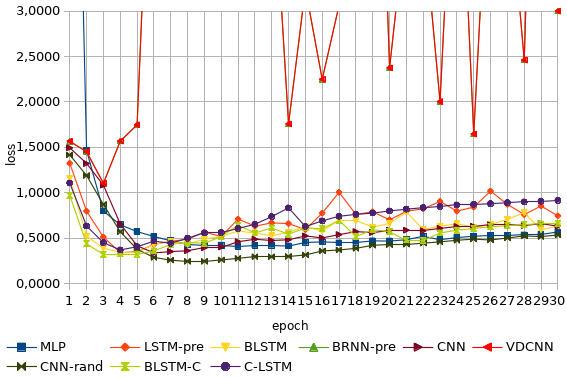
\includegraphics[width=\textwidth]{figuras/valloss}
        \caption{Conjunto de validação}
        \label{fig:valloss}
    \end{subfigure}
    \caption[\textit{Loss} dos modelos neurais]{\textit{Loss} dos modelos neurais durante a fase de treinamento e validação, separados por cada \textit{epoch}. Fonte: elaboração própria.}
    \label{fig:tvloss}
\end{figure}


Para os modelos neurais foram coletadas as informações de \textit{loss} e acurácia utilizados para parametrizar todas as redes, o resultado final da execução dos modelos com seus melhores parâmetros estão na Figura \ref{fig:tvacc} e \textit{loss} na Figura \ref{fig:tvloss}.

Foi realizado um corte nas Figuras \ref{fig:loss} e \ref{fig:valloss} para que as diferenças mais próximas dos intervalos de 0.5 e 0.01 do \textit{loss} se tornassem mais visíveis nos gráficos. Para o \textit{loss} no treino os valores nos \textit{epoch} de 1 a 9 para a BRNN que ficaram omitidas devido ao corte são: $3,3539$,	$3,7614$	$4,4127$, $4,6006$, $1,7363$, $1,1438$, $1,0280$, $1,8636$, $2,3836$. Pelo fato de se mostrar inconstante e sem tendência os erros da VDCNN, os valores no gráfico de \textit{loss} de validação não serão apresentados.

\subsection{Performance final}

Para a verdadeira avaliação da performance dos modelos, serão consideras as três métricas de revocação, precisão e acurácia apresentadas na Tabela \ref{tab:modelosMetricas}. Outra métrica a se levar em consideração é o tempo necessário para predizer as amostras do conjunto de teste, estes tempos são apresentados na Tabela \ref{tab:execucaoModelos}.

Para obter-se as métricas dos modelos CNN \cite{da_silva_document_2018} e BLSTMN \cite{braz_document_2018} que utilizaram o mesmo conjunto de dados, fez-se uso das matrizes de confusão na Figura \ref{fig:matrizSilva} e \ref{fig:matrizBraz} para o cálculo. Os resultados foram adicionados à Tabela \ref{tab:modelosMetricas}. 

\begin{figure}[ht]
    \centering
    \begin{subfigure}[b]{0.4\textwidth}
        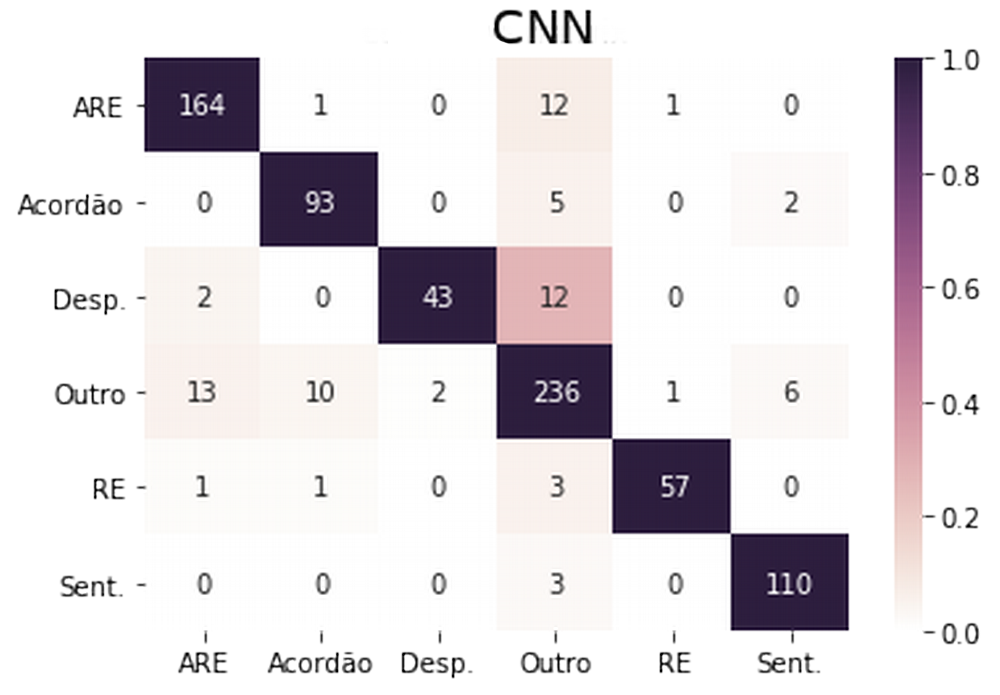
\includegraphics[width=\textwidth]{figuras/matrizSilva}
        \caption{Matriz de confusão CNN. Fonte: \cite[p. 3]{da_silva_document_2018}}
        \label{fig:matrizSilva}
    \end{subfigure}\hfill
    \begin{subfigure}[b]{0.45\textwidth}
        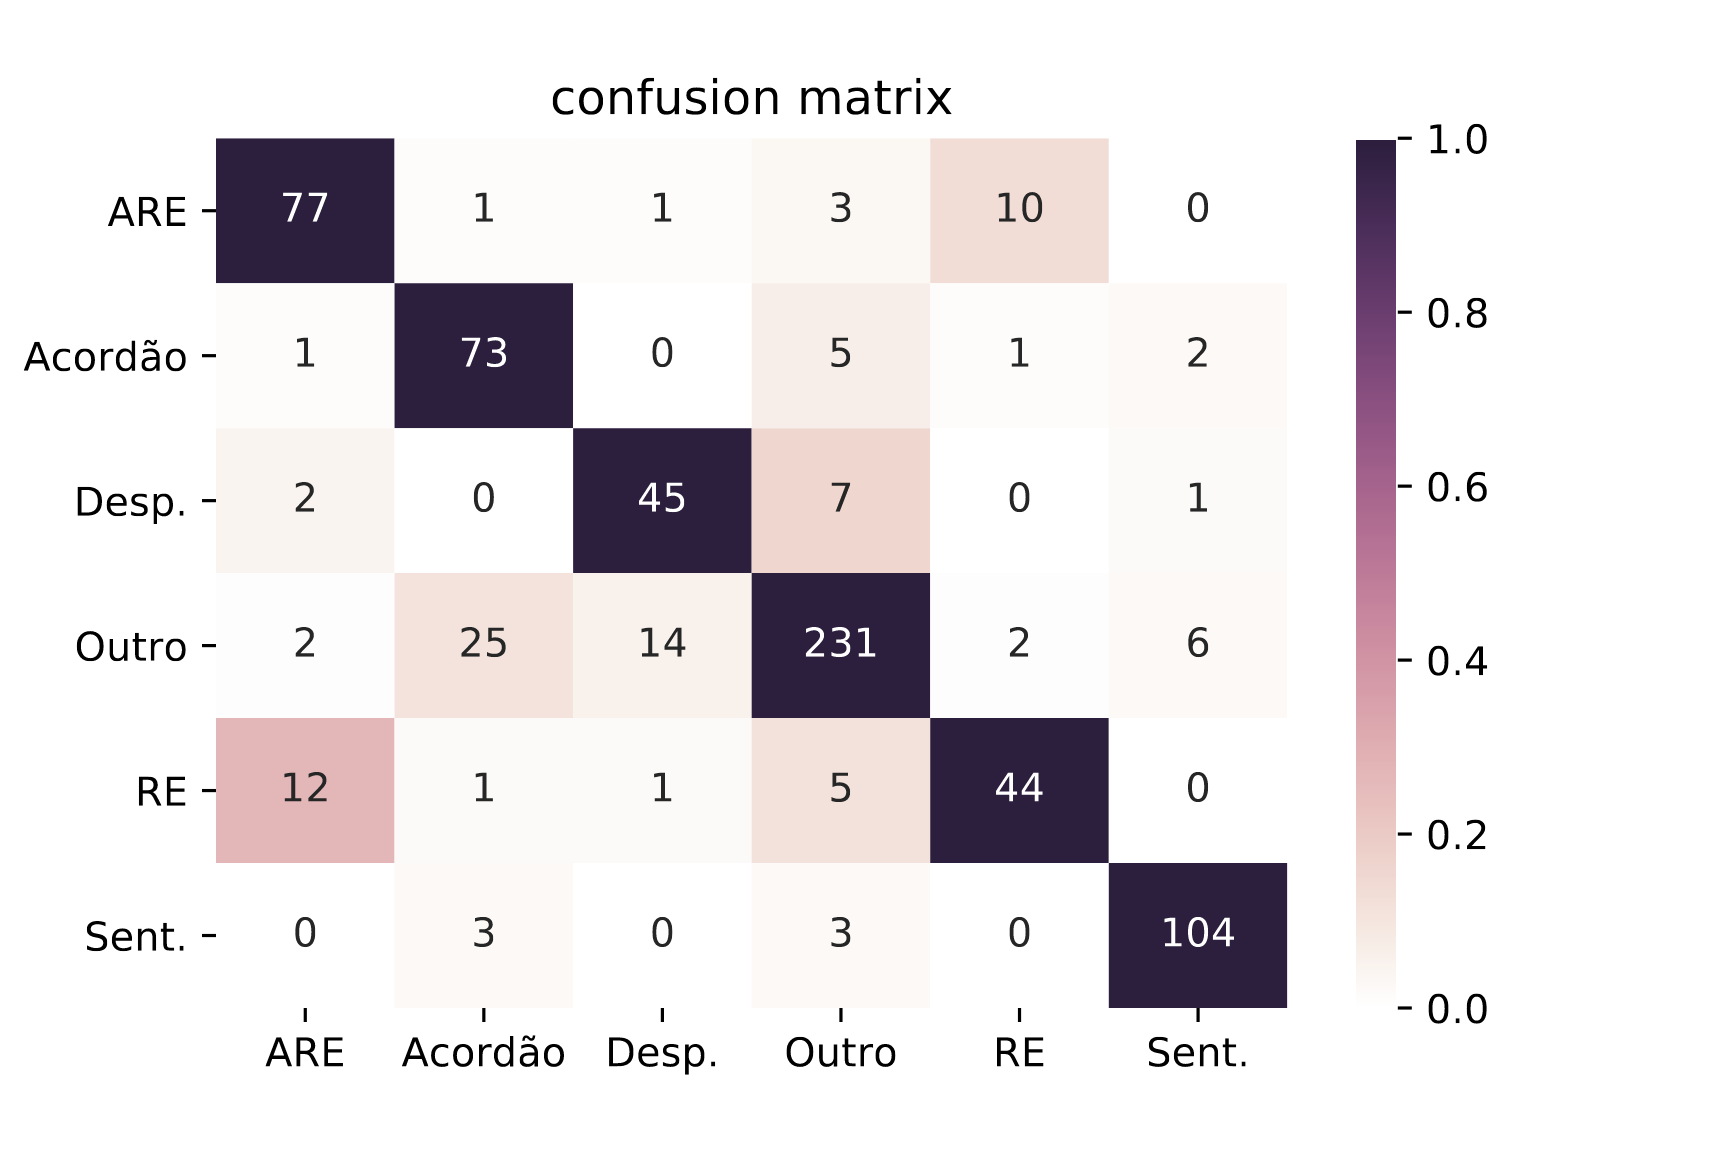
\includegraphics[width=\textwidth]{figuras/matrizBraz}
        \caption{Matriz de confusão BLSTM. Fonte: \cite[p. 3]{braz_document_2018}}
        \label{fig:matrizBraz}
    \end{subfigure}
    \caption[Matriz de confusão dos modelos CNN e BLSTM]{Matrizes de confusão para os modelos de CNN e BLSTM que utilizaram o mesmo conjunto de dados.}
\end{figure}

\begin{table}[ht]
    \centering
    \caption[Métricas dos modelos no conjunto de teste]{Métricas coletadas da execução de todos os modelos no conjunto de teste. Junto aos resultados obtidos por outros autores na mesma base de dados.}
    \label{tab:modelosMetricas}
    \begin{tabular}{|c|c|c|c|}
        \hline
        \textbf{Modelo} & \textbf{Acurácia} & \textbf{Precisão} & \textbf{Revocação} \\
        \hline
        DNN & 0,9164 & 0,9095 & 0,9258 \\ 
        \hline
        \textbf{LSTM-pre} & \textbf{0,9413} & \textbf{0,9334} & \textbf{0,9501} \\
        \hline
        BLSTM & 0,9326 & 0,9311 & 0,9289 \\ 
        \hline
        BRNN-pre & 0,8651 & 0,8428 & 0,8569 \\ 
        \hline
        CNN & 0,9326 & 0,9265 & 0,9316 \\ 
        \hline
        VDCNN & 0,8255 & 0,8153 & 0,8117 \\ 
        \hline
        CNN-rand & 0,9384 & 0,9286 & 0,9422 \\ 
        \hline
        BLSTM-C & 0,9179 & 0,9146 & 0,9201 \\ 
        \hline
        C-LSTM & 0,9208 & 0,9169 & 0,9168 \\
        \hline
        SVM Linear & 0,9311 & 0,9300 & 0,9277 \\ 
        \hline
        CNN \cite{da_silva_document_2018} & 0,9035 & 0,9202 & 0,8965 \\
        \hline
        BLSTM \cite{braz_document_2018} &	0,8416 & 0,8112 & 0,8357 \\
        \hline
    \end{tabular}\par Fonte: Elaboração própria.
\end{table}

Dos modelos neurais apresentados, apenas o VDCNN apresentou grandes oscilações na acurária e nos valores de \textit{loss}.  No conjunto de treino, a acurárcia dos modelos apresentavam bons resultados a partir da 10ª iteração, o que refletiu também no conjunto de validação. A partir deste ponto, percebe-se que eles começaram a indicar \textit{overfitting}, pois o \textit{loss} começou a aumentar na validação e se aproximar de 0 sem que houvessem mudanças significativas no valor da acurácia enquanto que na validação o \textit{loss} passou a aumentar.

A utilização das técnicas de pré-processamento mostraram diferença significativa apenas nos modelos recorrentes. Com o texto cru, os modelos não foram capaz de ajustar seus pesos para todas as classes. Com uma quantidade menor de símbolos presentes no texto, como apresentado na Tabela \ref{tab:metricasDocumentos}, foi possível que as características de memorização e adição de contexto fossem melhor aproveitadas.